\documentclass{article}


% if you need to pass options to natbib, use, e.g.:
%     \PassOptionsToPackage{numbers, compress}{natbib}
% before loading neurips_2023


% ready for submission
\usepackage[]{neurips_2023}


% to compile a preprint version, e.g., for submission to arXiv, add add the
% [preprint] option:
%     \usepackage[preprint]{neurips_2023}


% to compile a camera-ready version, add the [final] option, e.g.:
%     \usepackage[final]{neurips_2023}


% to avoid loading the natbib package, add option nonatbib:
%    \usepackage[nonatbib]{neurips_2023}


\usepackage[utf8]{inputenc} % allow utf-8 input
\usepackage[T1]{fontenc}    % use 8-bit T1 fonts
\usepackage{hyperref}       % hyperlinks
\usepackage{url}            % simple URL typesetting
\usepackage{booktabs}       % professional-quality tables
\usepackage{amsfonts}       % blackboard math symbols
\usepackage{nicefrac}       % compact symbols for 1/2, etc.
\usepackage{microtype}      % microtypography
\usepackage{xcolor}         % colors
\usepackage{multirow}
\usepackage{graphicx}       % include images
\usepackage{caption}

% Images folder


\title{Unsupervised Domain Adaptation}


% The \author macro works with any number of authors. There are two commands
% used to separate the names and addresses of multiple authors: \And and \AND.
%
% Using \And between authors leaves it to LaTeX to determine where to break the
% lines. Using \AND forces a line break at that point. So, if LaTeX puts 3 of 4
% authors names on the first line, and the last on the second line, try using
% \AND instead of \And before the third author name.


\author{ Krishna Agarwal\\%\thanks{Use footnote for providing further information
    %about author (webpage, alternative address)---\emph{not} for acknowledging
    %funding agencies.} \\
  Indian Institute of Science, Bangalore\\
  \texttt{krishnaagarw@iisc.ac.in} \\
  % examples of more authors
   \And
  {Pratham Gupta} \\
  Indian Institute of Science, Bangalore\\
  \texttt{prathamgupta@iisc.ac.in} \\
   \And
   {Gavish Bansal} \\
   Indian Institute of Science, Bangalore\\
   \texttt{gavishbansal@iisc.ac.in} \\
   \And
   {Kintan Saha} \\
   Indian Institute of Science, Bangalore\\
   \texttt{kintansaha@iisc.ac.in} \\
  % \And
  % Coauthor \\
  % Affiliation \\
  % Address \\
  % \texttt{email} \\
}


\begin{document}
\graphicspath{{./images/}}

\maketitle


\begin{abstract}
  
\end{abstract}


\section{Introduction}
Unsupervised domain adaptation (UDA) is a type of domain adaptation in machine learning where a model is trained on a source domain with labelled data, and then adapted to a target domain with unlabelled data.
In UDA, the source domain and target domain have different distributions, but
the goal is to leverage the labelled data in the source domain to improve performance on the target
domain. \\
This report is product of our exploration of state of the art UDA algorithms and their applications in various fields like computer vision, natural language processing, etc. 
We have reproduced the results of these key papers [] in this research area of machine learning.

\section{Methodology}

\subsection{Algorithms}
We have implemented the following algorithms for our experiments:
\begin{itemize}
  \item \textbf{DANN (Domain-Adversarial Neural Network)}[]: Trains the model in an adversarial manner to learn the domain invariant features using a gradient reversal layer and a DNN.
  \item \textbf{CORAL (Correlation Alignment), DeepCORAL}[][]: CORAL aligns the second-order statistics (covariances) of source and target features. Accordingly, DeepCORAL is an extension of CORAL that integrates correlation alignment into deep neural networks.
  \item \textbf{MMD (Maximum Mean Discrepancy)}[]: A metric that quantifies non-alignment between the source and target distributions. It is used as a loss function and in validating models. 
  \item \textbf{DSN (Domain Separation Network)}[]: Separates domain-specific and domain-invariant features for better adaptation. A state of the art method for domain invariant feature learning.
  \item \textbf{ATT (Adversarial Training with Triplet loss)}[]:An ensemble method that utilize two classifier trained on source domain to pseudo-label target domain to learn a classifier for it.
\end{itemize}

\subsection{Datasets}
We have used the following datasets\ref{tab:datasets} for our experiments:
\begin{table}[h]
  \centering
  \caption{Benchmark datasets used in our experiments.}
  \label{tab:datasets}
  \begin{tabular}{ll}
      \toprule
      \textbf{Dataset Category} & \textbf{Datasets} \\
      \midrule
      Computer Vision (Numbers)     & MNIST, MNIST-M, SVHN \\
      Computer Vision (Categorical) & Office: Amazon, DSLR, Webcam \\
      Sentiment Analysis (Classification)  & Amazon Review Sentiment \\
      \bottomrule
  \end{tabular}
\end{table}


\section{Experiments}
\subsection{CORAL and DeepCORAL}
\subsubsection{CORAL}

\subsubsection{DeepCORAL}
We have implemented the DeepCORAL algorithm and observed its performance in domain adaptation using the Office dataset, taking every combination of domains as source and target. The results are shown in Table \ref{tab:deepcoral}. Note that we also compare our results with the results mentioned in the survey paper[]. It is observable that the result for \textbf{W}$\rightarrow$ \textbf{A} is in disagreement with the result in the survey paper by approximately 4\%. The plausible reasons for this discrepancy have been mentioned in the Appendix.
 
\begin{table*}
  \caption{Classification accuracy (source $\rightarrow$ target) of DeepCORAL on the Office computer vision dataset.}
  \label{comparePerformance2}
  \begin{scriptsize}
  \begin{center}
  {\renewcommand{\arraystretch}{1.4}
  \begin{tabular}{@{}l cccccc@{}}
  \toprule
  \multicolumn{1}{c}{\multirow{2}{*}{\textbf{Result Source}}} & \multicolumn{6}{c}{\textbf{Office (Amazon, DSLR, Webcam)}} \\
  \cmidrule{2-7}
   & \textbf{A $\rightarrow$ W} & \textbf{D $\rightarrow$ W} & \textbf{W $\rightarrow$ D} & \textbf{A $\rightarrow$ D} & \textbf{D $\rightarrow$ A} & \textbf{W $\rightarrow$ A} \\
  \midrule
  \textbf{Our Code} & 62.05 & 95.32 & 99.56 & 64.44 & 52.77 & 56.49\\
  \hline
  \textbf{Survey Paper} & 66.4$\pm$0.4 & 95.7$\pm$0.3 & 99.2$\pm$0.1 & 66.8$\pm$0.6 & 52.8$\pm$0.2 & 51.5$\pm$0.3\\
  \bottomrule
  \end{tabular}
  }
  \end{center}
  \end{scriptsize}
  \label{tab:deepcoral}
\end{table*}

\subsection{Maximum Mean Discrepancy}
Similar to DeepCORAL, we also experimented by taking MMD as our divergence metric. We have used synthetic dataset to test the performance of MMD and it showed good good ability to adapt as shown in figure \ref{fig:mmd}. We empirically verified MMD's ability to distinguish between different distributions \ref{fig:mmd_power}. By testing on synthetically generated data\ref{fig:mmd_example}. 

\begin{figure}
  \centering
  \begin{minipage}{0.3\textwidth}
    \centering
    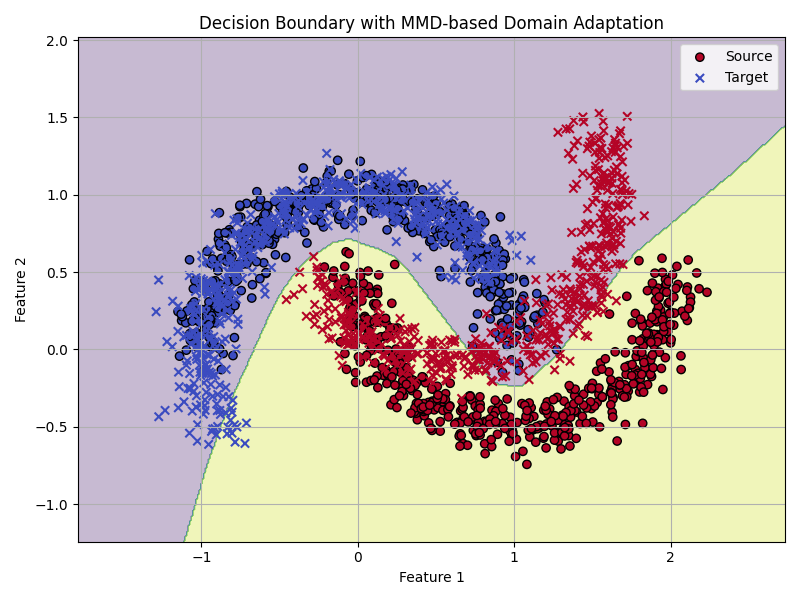
\includegraphics[width=\textwidth]{MMD/adaptation.png}
    \caption{Plot of desicion boundary of DNN trained with MMD loss. The decision boundary is shown for the source domain (dots) and target domain (cross).}
    \label{fig:mmd}
  \end{minipage}
  \hfill
  \begin{minipage}{0.35\textwidth}
    \centering
    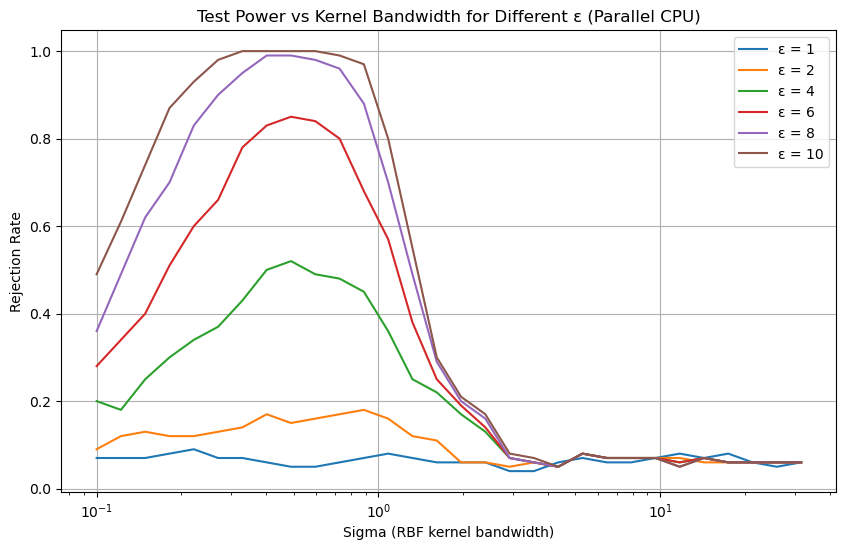
\includegraphics[width=\textwidth]{MMD/Test_powe_vs_eps.png}
    \caption{MMD: Test power vs epsilon shows how well MMD can distinguish between distributions vs how much they differ.}
    \label{fig:mmd_power}
  \end{minipage}
  \hfill
  \begin{minipage}{0.25\textwidth}
    \centering
    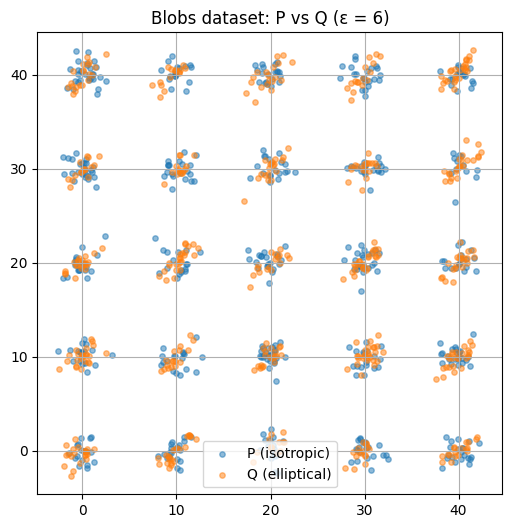
\includegraphics[width=\textwidth]{MMD/Example.png}
    \caption{Example of synthetic dataset, where P is Isotropic Gaussian while Q is elliptical.}
    \label{fig:mmd_example}
  \end{minipage}
  

\end{figure}


\subsection{Domain Separation Network}
We have implemented the DSN algorithm and observed its performance in domain adaptation using the MNIST and MNIST-M datasets. Our Resulting accuracy is shown in Table \ref{tab:dsn}. The results are comparable to the results mentioned in the paper. Further more we can also observe the reconstructed images from the DSN model. The reconstructed images are shown in figure \ref{fig:dsn_reconstruction}.




\begin{figure}
  \centering
  % First minipage: the table
  \begin{minipage}[t]{0.45\textwidth}
    \centering
    \begin{minipage}[t]{0.95\textwidth}
      \centering
      \captionof{table}{Results of DSN on MNIST and MNIST-M Domain Adaptation.}
      \label{tab:dsn}
      \begin{tabular}{lc}
        \toprule
        \textbf{Method} & \textbf{Accuracy} \\
        \midrule
        DSN (Ours) & 81.6\% \\
        DSN (Paper) & 83.2\% \\
        \bottomrule
      \end{tabular}
    \end{minipage}
    \vspace{2mm}
    \begin{minipage}[t]{0.95\textwidth}
      \vspace{4mm}
      \centering
      \begin{minipage}[t]{0.95\textwidth}
        \centering
        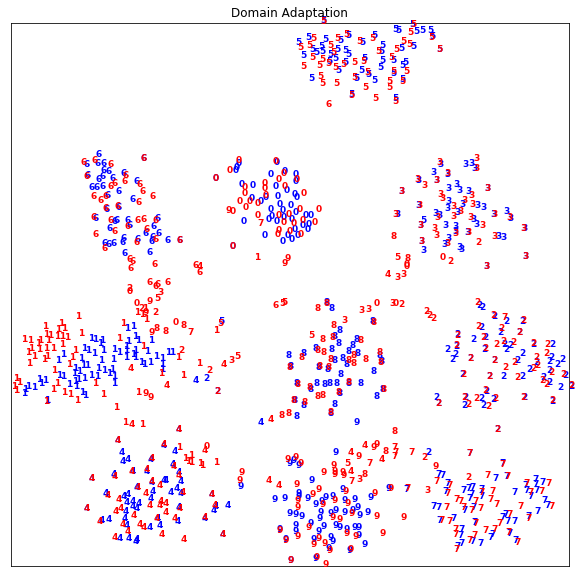
\includegraphics[width=0.75
        \linewidth]{DSN/DNS_MNIST_MNISTM.png}
        \caption{@krishna Put the caption here}
      \end{minipage}
    \end{minipage}
  \end{minipage}%
  \hfill
  % Second minipage: the 2x2 image grid
  \begin{minipage}[t]{0.5\textwidth}
    \caption{Reconstructed images from DSN.}
    \label{fig:dsn_reconstruction}
    \centering
    \begin{minipage}[t]{0.48\textwidth}
      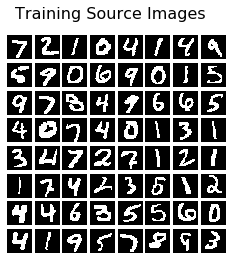
\includegraphics[width=\linewidth]{DSN/source.png}
    \end{minipage}
    \hfill
    \begin{minipage}[t]{0.48\textwidth}
      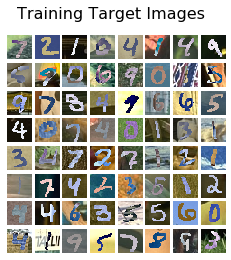
\includegraphics[width=\linewidth]{DSN/target.png}
    \end{minipage}
    \vspace{2mm}
    \begin{minipage}[t]{0.48\textwidth}
      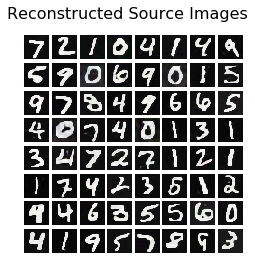
\includegraphics[width=\linewidth]{DSN/reconstructed_source.png}
    \end{minipage}
    \hfill
    \begin{minipage}[t]{0.48\textwidth}
      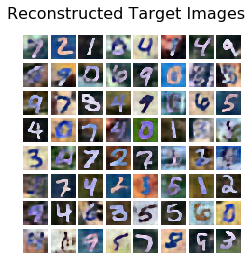
\includegraphics[width=\linewidth]{DSN/reconstructed_target.png}
    \end{minipage}

  \end{minipage}
\end{figure}



\subsection{Asymmetric Tri-training for Unsupervised Domain Adaptation}
We have Implement Asymmetric Tri-Training Algorithm and Tested it on MNIST and SVHN datasets. Results are shown in Table \ref{tab:att_results}. The results are comparable to the results mentioned in the paper. We have also compared our implementation with the implementation of the paper. The results are shown in Table \ref{tab:att_results}. It is observable that our implementation closely matched for training without batch normalization but other experiments then match the implementation of the paper. The plausible reasons for this discrepancy have been mentioned in the Appendix.
\begin{table}
  \centering
  \caption{Results of ATT on MNIST and SVHN Domain Adaptation.}
  \label{tab:att_results}
  \begin{tabular}{lccc}
      \toprule
      \textbf{Method} & \textbf{MNIST\(\to\)SVHN} & \textbf{SVHN \(\to\) MNIST} \\
      \midrule
      Our w/o Batch Normalization & 36.9\% & 76.8\% \\
      Ours w/o Multi-view Loss & 15.2\% & 76.5\% \\
      Ours  & 15.2\% & 71.4\% \\
      \midrule
      Papers w/o Batch Normalization & 39.8\% & 79.8\% \\
      Papers w/o Multi-view Loss & 49.7\% & 86.0\% \\
      Papers  & 52.8\% & 85.8\% \\
      \bottomrule
  \end{tabular}
\end{table}


% \begin{figure}[h]
%   \centering
%   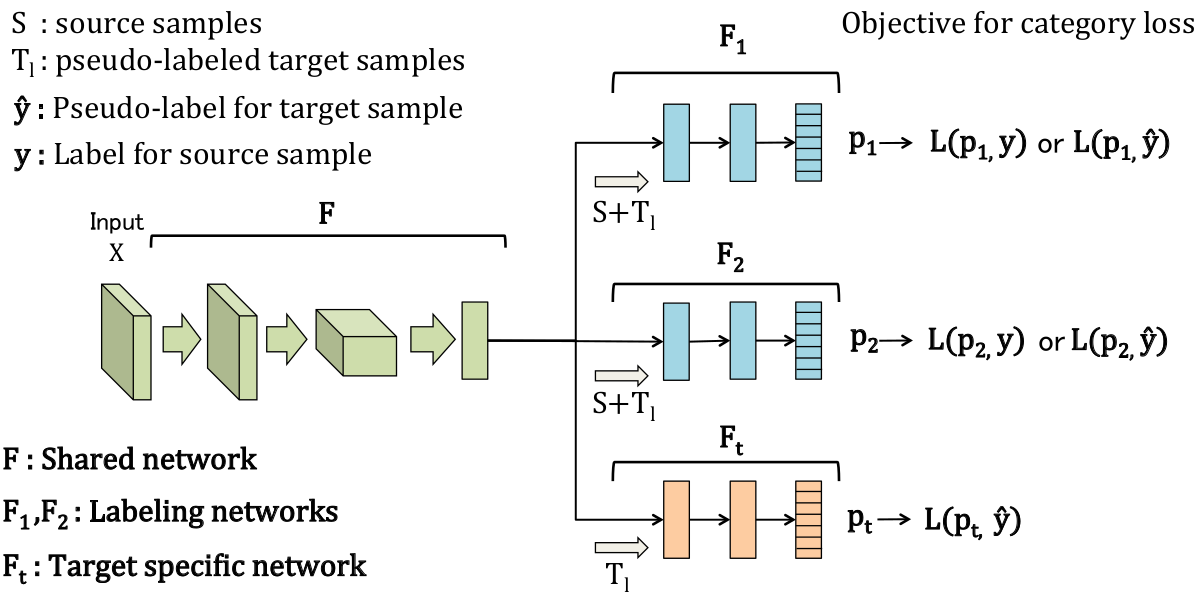
\includegraphics[width=0.5\textwidth]{ATT_Architecture.png}
%   \caption{ATT Architecture: The feature extractor F takes input from both source and target domain. F1 and F2 are classifiers trained on source domain. Ft is trained on target domain using pseudo-labels from F1 and F2.}
%   \label{fig:att_architecture}
% \end{figure}



\section{Conclusion}


\section*{Appendix}



%%%%%%%%%%%%%%%%%%%%%%%%%%%%%%%%%%%%%%%%%%%%%%%%%%%%%%%%%%%%


\end{document}